\documentclass[]{article}
\usepackage{lmodern}
\usepackage{amssymb,amsmath}
\usepackage{ifxetex,ifluatex}
\usepackage{fixltx2e} % provides \textsubscript
\ifnum 0\ifxetex 1\fi\ifluatex 1\fi=0 % if pdftex
  \usepackage[T1]{fontenc}
  \usepackage[utf8]{inputenc}
\else % if luatex or xelatex
  \ifxetex
    \usepackage{mathspec}
  \else
    \usepackage{fontspec}
  \fi
  \defaultfontfeatures{Ligatures=TeX,Scale=MatchLowercase}
\fi
% use upquote if available, for straight quotes in verbatim environments
\IfFileExists{upquote.sty}{\usepackage{upquote}}{}
% use microtype if available
\IfFileExists{microtype.sty}{%
\usepackage{microtype}
\UseMicrotypeSet[protrusion]{basicmath} % disable protrusion for tt fonts
}{}
\usepackage[margin=1in]{geometry}
\usepackage{hyperref}
\hypersetup{unicode=true,
            pdftitle={Summary Graphs of NUTR630 Intake},
            pdfauthor={Dave Bridges, Liv Anderson and Noura El Habbal},
            pdfborder={0 0 0},
            breaklinks=true}
\urlstyle{same}  % don't use monospace font for urls
\usepackage{color}
\usepackage{fancyvrb}
\newcommand{\VerbBar}{|}
\newcommand{\VERB}{\Verb[commandchars=\\\{\}]}
\DefineVerbatimEnvironment{Highlighting}{Verbatim}{commandchars=\\\{\}}
% Add ',fontsize=\small' for more characters per line
\usepackage{framed}
\definecolor{shadecolor}{RGB}{248,248,248}
\newenvironment{Shaded}{\begin{snugshade}}{\end{snugshade}}
\newcommand{\KeywordTok}[1]{\textcolor[rgb]{0.13,0.29,0.53}{\textbf{#1}}}
\newcommand{\DataTypeTok}[1]{\textcolor[rgb]{0.13,0.29,0.53}{#1}}
\newcommand{\DecValTok}[1]{\textcolor[rgb]{0.00,0.00,0.81}{#1}}
\newcommand{\BaseNTok}[1]{\textcolor[rgb]{0.00,0.00,0.81}{#1}}
\newcommand{\FloatTok}[1]{\textcolor[rgb]{0.00,0.00,0.81}{#1}}
\newcommand{\ConstantTok}[1]{\textcolor[rgb]{0.00,0.00,0.00}{#1}}
\newcommand{\CharTok}[1]{\textcolor[rgb]{0.31,0.60,0.02}{#1}}
\newcommand{\SpecialCharTok}[1]{\textcolor[rgb]{0.00,0.00,0.00}{#1}}
\newcommand{\StringTok}[1]{\textcolor[rgb]{0.31,0.60,0.02}{#1}}
\newcommand{\VerbatimStringTok}[1]{\textcolor[rgb]{0.31,0.60,0.02}{#1}}
\newcommand{\SpecialStringTok}[1]{\textcolor[rgb]{0.31,0.60,0.02}{#1}}
\newcommand{\ImportTok}[1]{#1}
\newcommand{\CommentTok}[1]{\textcolor[rgb]{0.56,0.35,0.01}{\textit{#1}}}
\newcommand{\DocumentationTok}[1]{\textcolor[rgb]{0.56,0.35,0.01}{\textbf{\textit{#1}}}}
\newcommand{\AnnotationTok}[1]{\textcolor[rgb]{0.56,0.35,0.01}{\textbf{\textit{#1}}}}
\newcommand{\CommentVarTok}[1]{\textcolor[rgb]{0.56,0.35,0.01}{\textbf{\textit{#1}}}}
\newcommand{\OtherTok}[1]{\textcolor[rgb]{0.56,0.35,0.01}{#1}}
\newcommand{\FunctionTok}[1]{\textcolor[rgb]{0.00,0.00,0.00}{#1}}
\newcommand{\VariableTok}[1]{\textcolor[rgb]{0.00,0.00,0.00}{#1}}
\newcommand{\ControlFlowTok}[1]{\textcolor[rgb]{0.13,0.29,0.53}{\textbf{#1}}}
\newcommand{\OperatorTok}[1]{\textcolor[rgb]{0.81,0.36,0.00}{\textbf{#1}}}
\newcommand{\BuiltInTok}[1]{#1}
\newcommand{\ExtensionTok}[1]{#1}
\newcommand{\PreprocessorTok}[1]{\textcolor[rgb]{0.56,0.35,0.01}{\textit{#1}}}
\newcommand{\AttributeTok}[1]{\textcolor[rgb]{0.77,0.63,0.00}{#1}}
\newcommand{\RegionMarkerTok}[1]{#1}
\newcommand{\InformationTok}[1]{\textcolor[rgb]{0.56,0.35,0.01}{\textbf{\textit{#1}}}}
\newcommand{\WarningTok}[1]{\textcolor[rgb]{0.56,0.35,0.01}{\textbf{\textit{#1}}}}
\newcommand{\AlertTok}[1]{\textcolor[rgb]{0.94,0.16,0.16}{#1}}
\newcommand{\ErrorTok}[1]{\textcolor[rgb]{0.64,0.00,0.00}{\textbf{#1}}}
\newcommand{\NormalTok}[1]{#1}
\usepackage{graphicx,grffile}
\makeatletter
\def\maxwidth{\ifdim\Gin@nat@width>\linewidth\linewidth\else\Gin@nat@width\fi}
\def\maxheight{\ifdim\Gin@nat@height>\textheight\textheight\else\Gin@nat@height\fi}
\makeatother
% Scale images if necessary, so that they will not overflow the page
% margins by default, and it is still possible to overwrite the defaults
% using explicit options in \includegraphics[width, height, ...]{}
\setkeys{Gin}{width=\maxwidth,height=\maxheight,keepaspectratio}
\IfFileExists{parskip.sty}{%
\usepackage{parskip}
}{% else
\setlength{\parindent}{0pt}
\setlength{\parskip}{6pt plus 2pt minus 1pt}
}
\setlength{\emergencystretch}{3em}  % prevent overfull lines
\providecommand{\tightlist}{%
  \setlength{\itemsep}{0pt}\setlength{\parskip}{0pt}}
\setcounter{secnumdepth}{0}
% Redefines (sub)paragraphs to behave more like sections
\ifx\paragraph\undefined\else
\let\oldparagraph\paragraph
\renewcommand{\paragraph}[1]{\oldparagraph{#1}\mbox{}}
\fi
\ifx\subparagraph\undefined\else
\let\oldsubparagraph\subparagraph
\renewcommand{\subparagraph}[1]{\oldsubparagraph{#1}\mbox{}}
\fi

%%% Use protect on footnotes to avoid problems with footnotes in titles
\let\rmarkdownfootnote\footnote%
\def\footnote{\protect\rmarkdownfootnote}

%%% Change title format to be more compact
\usepackage{titling}

% Create subtitle command for use in maketitle
\newcommand{\subtitle}[1]{
  \posttitle{
    \begin{center}\large#1\end{center}
    }
}

\setlength{\droptitle}{-2em}

  \title{Summary Graphs of NUTR630 Intake}
    \pretitle{\vspace{\droptitle}\centering\huge}
  \posttitle{\par}
    \author{Dave Bridges, Liv Anderson and Noura El Habbal}
    \preauthor{\centering\large\emph}
  \postauthor{\par}
      \predate{\centering\large\emph}
  \postdate{\par}
    \date{Septembe 3, 2018}


\begin{document}
\maketitle

{
\setcounter{tocdepth}{2}
\tableofcontents
}
\begin{Shaded}
\begin{Highlighting}[]
\KeywordTok{library}\NormalTok{(readr)}
\NormalTok{filename <-}\StringTok{ 'https://docs.google.com/spreadsheets/d/e/2PACX-1vSDRxu3Ur53iZVsg5Gg9nArNiKY2-xguRzoeWl-wQ5Ky8qxRGnuXXMWSReSF1tR_SU6dmcBTgb-cQiY/pub?gid=830256665&single=true&output=csv'}
\NormalTok{data <-}\StringTok{ }\KeywordTok{read_csv}\NormalTok{(filename)}
\end{Highlighting}
\end{Shaded}

These data can be found in
/Users/davebrid/Documents/GitHub/TeachingLectures/Michigan/NUTR630/Evaluation/Pre-Semester
Survey/2018 in a file named
\url{https://docs.google.com/spreadsheets/d/e/2PACX-1vSDRxu3Ur53iZVsg5Gg9nArNiKY2-xguRzoeWl-wQ5Ky8qxRGnuXXMWSReSF1tR_SU6dmcBTgb-cQiY/pub?gid=830256665\&single=true\&output=csv}.
This script was most recently updated on Wed Sep 5 10:24:41 2018.

\section{Analysis}\label{analysis}

\subsection{What Majors}\label{what-majors}

\begin{Shaded}
\begin{Highlighting}[]
\KeywordTok{library}\NormalTok{(forcats)}
\CommentTok{#grouped with most common 4}

\NormalTok{count.majors <-}
\StringTok{  }\NormalTok{data }\OperatorTok
\StringTok{  }\KeywordTok{mutate}\NormalTok{(}\StringTok{`}\DataTypeTok{Which discipline most closely matches your undergraduate degree?}\StringTok{`}\NormalTok{ =}\StringTok{ }\KeywordTok{fct_lump}\NormalTok{(}\KeywordTok{as.factor}\NormalTok{(data}\OperatorTok{$}\StringTok{`}\DataTypeTok{Which discipline most closely matches your undergraduate degree?}\StringTok{`}\NormalTok{), }\DataTypeTok{n=}\DecValTok{4}\NormalTok{)) }\OperatorTok
\StringTok{  }\KeywordTok{mutate}\NormalTok{(}\StringTok{`}\DataTypeTok{Which discipline most closely matches your undergraduate degree?}\StringTok{`}\NormalTok{ =}\StringTok{ }
\StringTok{           }\KeywordTok{fct_recode}\NormalTok{(}\StringTok{`}\DataTypeTok{Which discipline most closely matches your undergraduate degree?}\StringTok{`}\NormalTok{, }
                      \StringTok{"Neuroscience"}\NormalTok{ =}\StringTok{ "Psychology-related (Psychology, Neuroscience, etc.)"}\NormalTok{,}
                      \StringTok{"Nutrition"}\NormalTok{ =}\StringTok{ "Food Quality & Safety"}\NormalTok{,}
                      \StringTok{"Nutrition"}\NormalTok{ =}\StringTok{ "Nutrition & dietetics (minor in biology)"}\NormalTok{,}
                      \StringTok{"Nutrition"}\NormalTok{ =}\StringTok{ "Dietetics"}\NormalTok{,}
                      \StringTok{"Nutrition"}\NormalTok{ =}\StringTok{ "Nutrition and Food Science"}\NormalTok{,}
                      \StringTok{"Nutrition"}\NormalTok{ =}\StringTok{ "Food & Nutritional Sciences"}\NormalTok{,}
                      \StringTok{"Biological Sciences"}\NormalTok{ =}\StringTok{ "Biochemistry"}\NormalTok{,}
                      \StringTok{"Humanities"}\NormalTok{ =}\StringTok{ "English Lit and Commuications, years later I took biochem pre-reqs for my program"}\NormalTok{)) }\OperatorTok
\StringTok{  }\KeywordTok{group_by}\NormalTok{(}\StringTok{`}\DataTypeTok{Which discipline most closely matches your undergraduate degree?}\StringTok{`}\NormalTok{) }\OperatorTok
\StringTok{  }\KeywordTok{count}\NormalTok{() }\OperatorTok
\StringTok{  }\KeywordTok{arrange}\NormalTok{(}\KeywordTok{desc}\NormalTok{(n)) }
  
\KeywordTok{with}\NormalTok{(count.majors, }\KeywordTok{barplot}\NormalTok{(n,}
                          \DataTypeTok{las=}\DecValTok{1}\NormalTok{,}
                          \DataTypeTok{cex.names=}\FloatTok{0.66}\NormalTok{,}
                          \DataTypeTok{main=}\StringTok{"What was your major?"}\NormalTok{,}
                          \DataTypeTok{col=}\NormalTok{color.scheme,}
                          \DataTypeTok{names.arg=}\StringTok{`}\DataTypeTok{Which discipline most closely matches your undergraduate degree?}\StringTok{`}\NormalTok{))}

\KeywordTok{library}\NormalTok{(ggplot2)}
\end{Highlighting}
\end{Shaded}

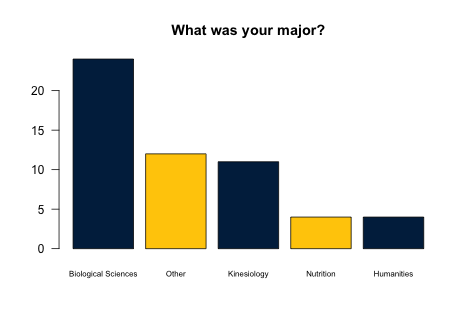
\includegraphics{figures/majors-summary-1.png}

\begin{Shaded}
\begin{Highlighting}[]
\KeywordTok{ggplot}\NormalTok{(count.majors,}\KeywordTok{aes}\NormalTok{(}\DataTypeTok{y=}\NormalTok{n,}\DataTypeTok{x=}\KeywordTok{reorder}\NormalTok{(}\StringTok{`}\DataTypeTok{Which discipline most closely matches your undergraduate degree?}\StringTok{`}\NormalTok{,}\OperatorTok{-}\NormalTok{n))) }\OperatorTok{+}
\StringTok{         }\KeywordTok{geom_bar}\NormalTok{(}\DataTypeTok{stat=}\StringTok{'identity'}\NormalTok{,}\DataTypeTok{fill=}\NormalTok{color.scheme[}\DecValTok{1}\NormalTok{]) }\OperatorTok{+}
\StringTok{  }\KeywordTok{labs}\NormalTok{(}\DataTypeTok{y=}\StringTok{"Number of Students"}\NormalTok{,}
       \DataTypeTok{title=}\StringTok{"Which discipline most closely matches your undergraduate degree?"}\NormalTok{,}
       \DataTypeTok{x=}\StringTok{""}\NormalTok{)}
\end{Highlighting}
\end{Shaded}

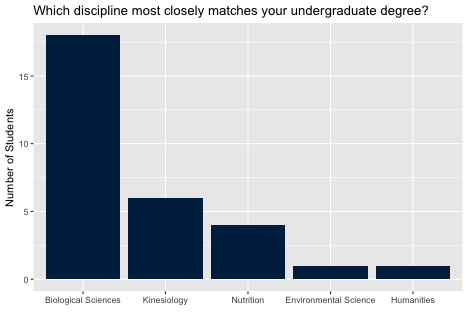
\includegraphics{figures/majors-summary-2.png}

\subsection{What Topics are Students Interested
In?}\label{what-topics-are-students-interested-in}

\begin{Shaded}
\begin{Highlighting}[]
\KeywordTok{library}\NormalTok{(sjPlot)}

\NormalTok{student.interest.data <-}\StringTok{ }
\StringTok{  }\NormalTok{data }\OperatorTok
\StringTok{  }\KeywordTok{select}\NormalTok{(}\KeywordTok{starts_with}\NormalTok{(}\StringTok{'Please answer these questions about your interests'}\NormalTok{)) }\OperatorTok
\StringTok{  }\KeywordTok{rename}\NormalTok{(}\StringTok{"Biochemistry - Interest"}\NormalTok{ =}\StringTok{ "Please answer these questions about your interests [Macronutrient biochemistry is of interest to me.]"}\NormalTok{,}
         \StringTok{"Biochemistry - Important"}\NormalTok{ =}\StringTok{ "Please answer these questions about your interests [Macronutrient biochemistry is important for my career interests.]"}\NormalTok{,}
         \StringTok{"Digestion - Interest"}\NormalTok{ =}\StringTok{ "Please answer these questions about your interests [Comprehensive understanding of the digestive tract is of interest to me.]"}\NormalTok{,}
         \StringTok{"Digestion - Important"}\NormalTok{ =}\StringTok{ "Please answer these questions about your interests [Comprehensive understanding of the digestive tract is important for my career interests.]"}\NormalTok{) }\OperatorTok
\StringTok{  }\KeywordTok{mutate}\NormalTok{(}\StringTok{`}\DataTypeTok{Biochemistry - Interest}\StringTok{`}\NormalTok{=}\StringTok{ }\KeywordTok{fct_recode}\NormalTok{(}\StringTok{`}\DataTypeTok{Biochemistry - Interest}\StringTok{`}\NormalTok{, }
                                                 \StringTok{'1'}\NormalTok{=}\StringTok{"Strongly Agree"}\NormalTok{,}
                                                 \StringTok{'2'}\NormalTok{=}\StringTok{"Agree"}\NormalTok{,}
                                                 \StringTok{'3'}\NormalTok{=}\StringTok{"Neutral"}\NormalTok{,}
                                                 \StringTok{'4'}\NormalTok{=}\StringTok{"Disagree"}\NormalTok{,}
                                                 \StringTok{'5'}\NormalTok{=}\StringTok{"Strongly Disagree"}\NormalTok{)) }\OperatorTok
\StringTok{  }\KeywordTok{mutate}\NormalTok{(}\StringTok{`}\DataTypeTok{Biochemistry - Important}\StringTok{`}\NormalTok{=}\StringTok{ }\KeywordTok{fct_recode}\NormalTok{(}\StringTok{`}\DataTypeTok{Biochemistry - Important}\StringTok{`}\NormalTok{, }
                                                 \StringTok{'1'}\NormalTok{=}\StringTok{"Strongly Agree"}\NormalTok{,}
                                                 \StringTok{'2'}\NormalTok{=}\StringTok{"Agree"}\NormalTok{,}
                                                 \StringTok{'3'}\NormalTok{=}\StringTok{"Neutral"}\NormalTok{,}
                                                 \StringTok{'4'}\NormalTok{=}\StringTok{"Disagree"}\NormalTok{,}
                                                 \StringTok{'5'}\NormalTok{=}\StringTok{"Strongly Disagree"}\NormalTok{)) }\OperatorTok
\StringTok{    }\KeywordTok{mutate}\NormalTok{(}\StringTok{`}\DataTypeTok{Digestion - Interest}\StringTok{`}\NormalTok{=}\StringTok{ }\KeywordTok{fct_recode}\NormalTok{(}\StringTok{`}\DataTypeTok{Digestion - Interest}\StringTok{`}\NormalTok{, }
                                                 \StringTok{'1'}\NormalTok{=}\StringTok{"Strongly Agree"}\NormalTok{,}
                                                 \StringTok{'2'}\NormalTok{=}\StringTok{"Agree"}\NormalTok{,}
                                                 \StringTok{'3'}\NormalTok{=}\StringTok{"Neutral"}\NormalTok{,}
                                                 \StringTok{'4'}\NormalTok{=}\StringTok{"Disagree"}\NormalTok{,}
                                                 \StringTok{'5'}\NormalTok{=}\StringTok{"Strongly Disagree"}\NormalTok{)) }\OperatorTok
\StringTok{      }\KeywordTok{mutate}\NormalTok{(}\StringTok{`}\DataTypeTok{Digestion - Important}\StringTok{`}\NormalTok{=}\StringTok{ }\KeywordTok{fct_recode}\NormalTok{(}\StringTok{`}\DataTypeTok{Digestion - Important}\StringTok{`}\NormalTok{, }
                                                 \StringTok{'1'}\NormalTok{=}\StringTok{"Strongly Agree"}\NormalTok{,}
                                                 \StringTok{'2'}\NormalTok{=}\StringTok{"Agree"}\NormalTok{,}
                                                 \StringTok{'3'}\NormalTok{=}\StringTok{"Neutral"}\NormalTok{,}
                                                 \StringTok{'4'}\NormalTok{=}\StringTok{"Disagree"}\NormalTok{,}
                                                 \StringTok{'5'}\NormalTok{=}\StringTok{"Strongly Disagree"}\NormalTok{)) }\OperatorTok
\StringTok{  }\KeywordTok{mutate}\NormalTok{(}\StringTok{`}\DataTypeTok{Biochemistry - Interest}\StringTok{`}\NormalTok{=}\KeywordTok{as.numeric}\NormalTok{(}\KeywordTok{as.character}\NormalTok{(}\StringTok{`}\DataTypeTok{Biochemistry - Interest}\StringTok{`}\NormalTok{))) }\OperatorTok
\StringTok{  }\KeywordTok{mutate}\NormalTok{(}\StringTok{`}\DataTypeTok{Biochemistry - Important}\StringTok{`}\NormalTok{=}\KeywordTok{as.numeric}\NormalTok{(}\KeywordTok{as.character}\NormalTok{(}\StringTok{`}\DataTypeTok{Biochemistry - Important}\StringTok{`}\NormalTok{))) }\OperatorTok
\StringTok{  }\KeywordTok{mutate}\NormalTok{(}\StringTok{`}\DataTypeTok{Digestion - Interest}\StringTok{`}\NormalTok{=}\KeywordTok{as.numeric}\NormalTok{(}\KeywordTok{as.character}\NormalTok{(}\StringTok{`}\DataTypeTok{Digestion - Interest}\StringTok{`}\NormalTok{))) }\OperatorTok
\StringTok{  }\KeywordTok{mutate}\NormalTok{(}\StringTok{`}\DataTypeTok{Digestion - Important}\StringTok{`}\NormalTok{=}\KeywordTok{as.numeric}\NormalTok{(}\KeywordTok{as.character}\NormalTok{(}\StringTok{`}\DataTypeTok{Digestion - Important}\StringTok{`}\NormalTok{))) }

\KeywordTok{plot_likert}\NormalTok{(student.interest.data,}
           \DataTypeTok{sort.frq=}\OtherTok{NULL}\NormalTok{,}
           \DataTypeTok{values=}\StringTok{'hide'}\NormalTok{,}
           \DataTypeTok{reverse.colors=}\OtherTok{TRUE}\NormalTok{,}
           \DataTypeTok{show.legend=}\OtherTok{FALSE}\NormalTok{,}
           \DataTypeTok{show.n=}\OtherTok{FALSE}\NormalTok{)}
\end{Highlighting}
\end{Shaded}

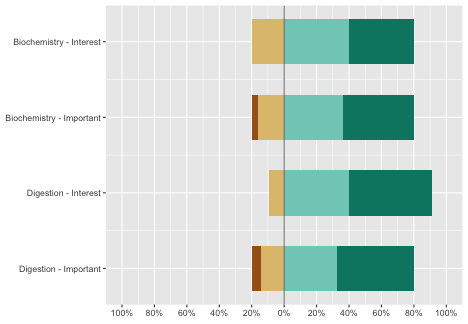
\includegraphics{figures/student-interests-1.png}

\subsubsection{What Topic are you Most Interested
In?}\label{what-topic-are-you-most-interested-in}

\begin{Shaded}
\begin{Highlighting}[]
\KeywordTok{library}\NormalTok{(stringr)}
\NormalTok{topic.interest <-}\StringTok{ }
\StringTok{  }\NormalTok{data }\OperatorTok
\StringTok{  }\KeywordTok{select}\NormalTok{(}\StringTok{`}\DataTypeTok{After reading the syllabus, which topic are you most excited to learn about?}\StringTok{`}\NormalTok{) }\OperatorTok
\StringTok{  }\KeywordTok{mutate}\NormalTok{(}\DataTypeTok{Interest =} \StringTok{`}\DataTypeTok{After reading the syllabus, which topic are you most excited to learn about?}\StringTok{`}\NormalTok{) }\OperatorTok
\StringTok{  }\KeywordTok{mutate}\NormalTok{(}\DataTypeTok{Microbiome =} \KeywordTok{ifelse}\NormalTok{(}\KeywordTok{str_detect}\NormalTok{(Interest, }\StringTok{"Microbiome|microbiome"}\NormalTok{), }\OtherTok{TRUE}\NormalTok{, }\OtherTok{FALSE}\NormalTok{),}
         \DataTypeTok{Fiber =} \KeywordTok{ifelse}\NormalTok{(}\KeywordTok{str_detect}\NormalTok{(Interest, }\StringTok{"Fiber|fibre"}\NormalTok{), }\OtherTok{TRUE}\NormalTok{, }\OtherTok{FALSE}\NormalTok{),}
         \DataTypeTok{Balance =} \KeywordTok{ifelse}\NormalTok{(}\KeywordTok{str_detect}\NormalTok{(Interest, }\StringTok{"balance|Balance"}\NormalTok{), }\OtherTok{TRUE}\NormalTok{, }\OtherTok{FALSE}\NormalTok{),}
         \DataTypeTok{Digestion =} \KeywordTok{ifelse}\NormalTok{(}\KeywordTok{str_detect}\NormalTok{(Interest, }\StringTok{"digest|Digest"}\NormalTok{), }\OtherTok{TRUE}\NormalTok{, }\OtherTok{FALSE}\NormalTok{),}
         \DataTypeTok{Biochem =} \KeywordTok{ifelse}\NormalTok{(}\KeywordTok{str_detect}\NormalTok{(Interest, }\StringTok{"biochem|Biochem"}\NormalTok{), }\OtherTok{TRUE}\NormalTok{, }\OtherTok{FALSE}\NormalTok{)) }\OperatorTok
\StringTok{  }\KeywordTok{select}\NormalTok{(Microbiome,Fiber,Balance,Digestion,Biochem) }\OperatorTok
\StringTok{  }\KeywordTok{gather}\NormalTok{(}\DataTypeTok{key=}\NormalTok{Interest, }\DataTypeTok{value=}\NormalTok{Response) }\OperatorTok
\StringTok{  }\KeywordTok{filter}\NormalTok{(Response}\OperatorTok{==}\OtherTok{TRUE}\NormalTok{) }\OperatorTok
\StringTok{  }\KeywordTok{count}\NormalTok{(Interest)}

\KeywordTok{ggplot}\NormalTok{(topic.interest, }\KeywordTok{aes}\NormalTok{(}\DataTypeTok{y=}\NormalTok{n,}\DataTypeTok{x=}\KeywordTok{reorder}\NormalTok{(Interest,n))) }\OperatorTok{+}
\StringTok{  }\KeywordTok{geom_bar}\NormalTok{(}\DataTypeTok{stat=}\StringTok{'identity'}\NormalTok{,}\DataTypeTok{fill=}\NormalTok{color.scheme[}\DecValTok{1}\NormalTok{]) }\OperatorTok{+}
\StringTok{  }\KeywordTok{coord_flip}\NormalTok{() }\OperatorTok{+}
\StringTok{  }\KeywordTok{labs}\NormalTok{(}\DataTypeTok{y=}\StringTok{'Number of Students'}\NormalTok{,}
       \DataTypeTok{x=}\StringTok{""}\NormalTok{,}
       \DataTypeTok{title=}\StringTok{""}\NormalTok{)}
\end{Highlighting}
\end{Shaded}

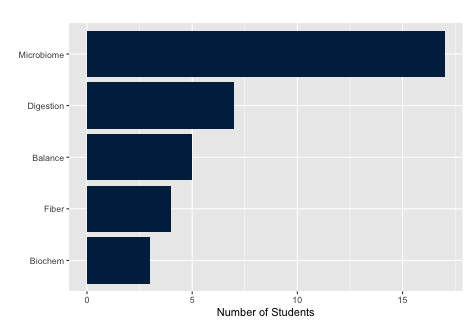
\includegraphics{figures/qualitative-interests-1.png}

\subsection{Applications of Course
Content}\label{applications-of-course-content}

\begin{Shaded}
\begin{Highlighting}[]
\KeywordTok{library}\NormalTok{(stringr)}
\NormalTok{application.data <-}\StringTok{ }
\StringTok{  }\NormalTok{data }\OperatorTok
\StringTok{  }\KeywordTok{select}\NormalTok{(}\StringTok{`}\DataTypeTok{What applications of this course content are you interested in?  Select all that apply.}\StringTok{`}\NormalTok{) }\OperatorTok
\StringTok{  }\KeywordTok{rename}\NormalTok{(}\DataTypeTok{Applications =} \StringTok{`}\DataTypeTok{What applications of this course content are you interested in?  Select all that apply.}\StringTok{`}\NormalTok{)}

\NormalTok{application.results =}\StringTok{ }\KeywordTok{str_split}\NormalTok{(application.data}\OperatorTok{$}\NormalTok{Applications, }\DataTypeTok{pattern=}\StringTok{', '}\NormalTok{, }\DataTypeTok{simplify =}\NormalTok{F) }\OperatorTok\StringTok{ }\KeywordTok{unlist}\NormalTok{() }

\NormalTok{application.summary <-}
\StringTok{  }\KeywordTok{as.data.frame}\NormalTok{(application.results) }\OperatorTok
\StringTok{  }\KeywordTok{rename}\NormalTok{(}\DataTypeTok{Results =}\NormalTok{ application.results) }\OperatorTok
\StringTok{  }\KeywordTok{count}\NormalTok{(Results) }\OperatorTok
\StringTok{  }\KeywordTok{arrange}\NormalTok{(n)}

\KeywordTok{ggplot}\NormalTok{(application.summary, }\KeywordTok{aes}\NormalTok{(}\DataTypeTok{y=}\NormalTok{n,}\DataTypeTok{x=}\KeywordTok{reorder}\NormalTok{(Results,n))) }\OperatorTok{+}
\StringTok{  }\KeywordTok{geom_bar}\NormalTok{(}\DataTypeTok{stat=}\StringTok{'identity'}\NormalTok{,}\DataTypeTok{fill=}\NormalTok{color.scheme[}\DecValTok{1}\NormalTok{]) }\OperatorTok{+}
\StringTok{  }\KeywordTok{coord_flip}\NormalTok{() }\OperatorTok{+}
\StringTok{  }\KeywordTok{labs}\NormalTok{(}\DataTypeTok{y=}\StringTok{'Number of Students'}\NormalTok{,}
       \DataTypeTok{x=}\StringTok{""}\NormalTok{,}
       \DataTypeTok{title=}\StringTok{""}\NormalTok{)}
\end{Highlighting}
\end{Shaded}

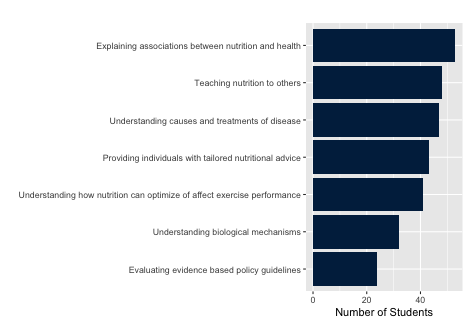
\includegraphics{figures/applications-content-1.png}

\section{Student Experience Data}\label{student-experience-data}

\begin{Shaded}
\begin{Highlighting}[]
\NormalTok{student.exp.data <-}
\StringTok{  }\NormalTok{data }\OperatorTok
\StringTok{  }\KeywordTok{select}\NormalTok{(}\StringTok{`}\DataTypeTok{I have previously written a literature review for a class.}\StringTok{`}\NormalTok{,}
\StringTok{`}\DataTypeTok{In college, have you ever done an in-class presentation?}\StringTok{`}\NormalTok{,}\StringTok{`}\DataTypeTok{Have you ever been asked to review a peer's presentation?}\StringTok{`}\NormalTok{,}\StringTok{`}\DataTypeTok{Have you ever been asked to evaluate a news article for class?}\StringTok{`}\NormalTok{,}\StringTok{`}\DataTypeTok{Have you ever written review questions based on material you were taught?}\StringTok{`}\NormalTok{)}

\NormalTok{countYes =}\StringTok{ }\ControlFlowTok{function}\NormalTok{(v)\{}\KeywordTok{length}\NormalTok{(v[v}\OperatorTok{==}\StringTok{"Yes"}\NormalTok{])\}}
\NormalTok{student.exp.data.summary <-}\StringTok{ }\KeywordTok{sapply}\NormalTok{(student.exp.data,countYes) }
\NormalTok{student.exp.data.summary <-}\StringTok{ }\KeywordTok{as_tibble}\NormalTok{(student.exp.data.summary)}
\NormalTok{student.exp.data.summary}\OperatorTok{$}\NormalTok{Question <-}\StringTok{ }\KeywordTok{rownames}\NormalTok{(student.exp.data.summary) }

\KeywordTok{ggplot}\NormalTok{(student.exp.data.summary, }\KeywordTok{aes}\NormalTok{(}\DataTypeTok{x=}\KeywordTok{reorder}\NormalTok{(Question,value),}\DataTypeTok{y=}\NormalTok{value}\OperatorTok{/}\KeywordTok{dim}\NormalTok{(student.exp.data)[}\DecValTok{1}\NormalTok{]}\OperatorTok{*}\DecValTok{100}\NormalTok{)) }\OperatorTok{+}
\StringTok{  }\KeywordTok{geom_bar}\NormalTok{(}\DataTypeTok{stat=}\StringTok{'identity'}\NormalTok{,}\DataTypeTok{fill=}\NormalTok{color.scheme[}\DecValTok{1}\NormalTok{]) }\OperatorTok{+}\StringTok{ }\KeywordTok{coord_flip}\NormalTok{() }\OperatorTok{+}
\StringTok{  }\KeywordTok{labs}\NormalTok{(}\DataTypeTok{x=}\StringTok{""}\NormalTok{,}\DataTypeTok{y=}\StringTok{"Percent"}\NormalTok{,}\DataTypeTok{title=}\StringTok{"Assignment Experiences"}\NormalTok{)}
\end{Highlighting}
\end{Shaded}

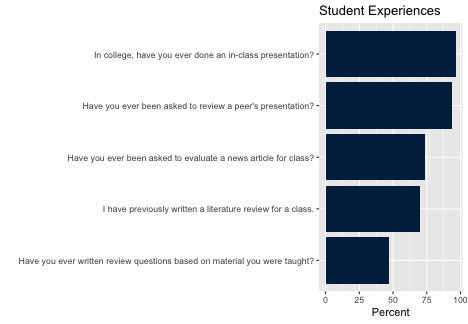
\includegraphics{figures/student-experience-1.png}

\subsection{Online Resources}\label{online-resources}

\begin{Shaded}
\begin{Highlighting}[]
\NormalTok{online.data <-}
\StringTok{  }\NormalTok{data }\OperatorTok
\StringTok{  }\KeywordTok{select}\NormalTok{(}\KeywordTok{starts_with}\NormalTok{(}\StringTok{"Which of the following online resources do you use for learning about nutrition?  Have you ever shared nutrition content in them?"}\NormalTok{))}
\KeywordTok{colnames}\NormalTok{(online.data) <-}\StringTok{ }\KeywordTok{gsub}\NormalTok{(}\StringTok{".*}\CharTok{\textbackslash{}\textbackslash{}}\StringTok{[|}\CharTok{\textbackslash{}\textbackslash{}}\StringTok{]"}\NormalTok{, }\StringTok{""}\NormalTok{, }\KeywordTok{colnames}\NormalTok{(online.data))}

\NormalTok{online.data.summary <-}
\StringTok{  }\KeywordTok{gather}\NormalTok{(online.data,}\DataTypeTok{key=}\StringTok{"Tool"}\NormalTok{,}\DataTypeTok{value=}\StringTok{"Use"}\NormalTok{) }\OperatorTok\StringTok{ }
\StringTok{  }\KeywordTok{group_by}\NormalTok{(Tool) }\OperatorTok\StringTok{ }
\StringTok{  }\KeywordTok{count}\NormalTok{(Use) }\OperatorTok
\StringTok{  }\NormalTok{na.omit }
  
\KeywordTok{ggplot}\NormalTok{(}\KeywordTok{filter}\NormalTok{(online.data.summary, Use }\OperatorTok{!=}\StringTok{ "Contributor"}\NormalTok{), }\KeywordTok{aes}\NormalTok{(}\DataTypeTok{y=}\NormalTok{n,}\DataTypeTok{x=}\KeywordTok{reorder}\NormalTok{(Tool,n))) }\OperatorTok{+}
\StringTok{  }\KeywordTok{geom_bar}\NormalTok{(}\DataTypeTok{stat=}\StringTok{'identity'}\NormalTok{,}\DataTypeTok{fill=}\NormalTok{color.scheme[}\DecValTok{1}\NormalTok{]) }\OperatorTok{+}
\StringTok{  }\KeywordTok{facet_grid}\NormalTok{(Use}\OperatorTok{~}\NormalTok{.) }\OperatorTok{+}
\StringTok{  }\KeywordTok{labs}\NormalTok{(}\DataTypeTok{y=}\StringTok{"Number of Students"}\NormalTok{,}\DataTypeTok{x=}\StringTok{""}\NormalTok{,}\DataTypeTok{title=}\StringTok{"Use of Online Resources"}\NormalTok{)}
\end{Highlighting}
\end{Shaded}

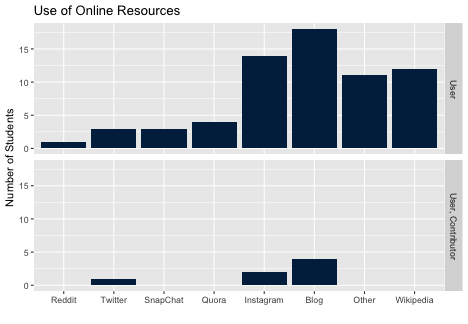
\includegraphics{figures/online-resources-1.png}

\subsection{GradeCraft Familiarity}\label{gradecraft-familiarity}

\begin{Shaded}
\begin{Highlighting}[]
\NormalTok{gradecraft <-}\StringTok{ }
\StringTok{  }\NormalTok{data }\OperatorTok
\StringTok{  }\KeywordTok{group_by}\NormalTok{(}\StringTok{`}\DataTypeTok{Are you familiar with GradeCraft?}\StringTok{`}\NormalTok{) }\OperatorTok
\StringTok{  }\KeywordTok{count}\NormalTok{()}

\KeywordTok{with}\NormalTok{(gradecraft, }\KeywordTok{barplot}\NormalTok{(n,}
                          \DataTypeTok{las=}\DecValTok{1}\NormalTok{,}
                          \DataTypeTok{ylab=}\StringTok{"Responses"}\NormalTok{,}
                          \DataTypeTok{main=}\StringTok{"Are you familiar with GradeCraft?"}\NormalTok{,}
                          \DataTypeTok{col=}\NormalTok{color.scheme,}
                          \DataTypeTok{names.arg=}\StringTok{`}\DataTypeTok{Are you familiar with GradeCraft?}\StringTok{`}\NormalTok{))}
\end{Highlighting}
\end{Shaded}

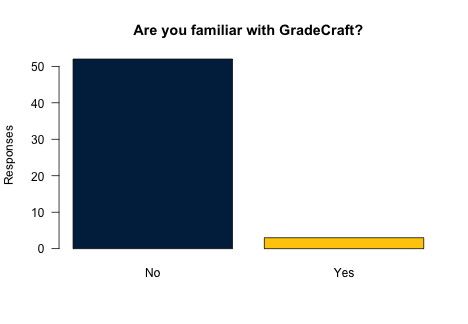
\includegraphics{figures/gradecraft-1.png}

Only 3 out of 55 students were familiar with GradeCraft.

\section{Session Information}\label{session-information}

\begin{Shaded}
\begin{Highlighting}[]
\KeywordTok{sessionInfo}\NormalTok{()}
\end{Highlighting}
\end{Shaded}

\begin{verbatim}
## R version 3.5.0 (2018-04-23)
## Platform: x86_64-apple-darwin15.6.0 (64-bit)
## Running under: macOS High Sierra 10.13.6
## 
## Matrix products: default
## BLAS: /Library/Frameworks/R.framework/Versions/3.5/Resources/lib/libRblas.0.dylib
## LAPACK: /Library/Frameworks/R.framework/Versions/3.5/Resources/lib/libRlapack.dylib
## 
## locale:
## [1] en_US.UTF-8/en_US.UTF-8/en_US.UTF-8/C/en_US.UTF-8/en_US.UTF-8
## 
## attached base packages:
## [1] stats     graphics  grDevices utils     datasets  methods   base     
## 
## other attached packages:
## [1] stringr_1.3.1  sjPlot_2.6.0   ggplot2_3.0.0  bindrcpp_0.2.2
## [5] forcats_0.3.0  readr_1.1.1    dplyr_0.7.6    tidyr_0.8.1   
## [9] knitr_1.20    
## 
## loaded via a namespace (and not attached):
##  [1] splines_3.5.0      carData_3.0-1      modelr_0.1.2      
##  [4] assertthat_0.2.0   stats4_3.5.0       coin_1.2-2        
##  [7] yaml_2.2.0         pillar_1.3.0       backports_1.1.2   
## [10] lattice_0.20-35    glue_1.3.0         digest_0.6.16     
## [13] RColorBrewer_1.1-2 glmmTMB_0.2.2.0    snakecase_0.9.2   
## [16] minqa_1.2.4        colorspace_1.3-2   sandwich_2.5-0    
## [19] psych_1.8.4        htmltools_0.3.6    Matrix_1.2-14     
## [22] survey_3.33-2      plyr_1.8.4         pkgconfig_2.0.2   
## [25] broom_0.5.0        haven_1.1.2        purrr_0.2.5       
## [28] xtable_1.8-2       mvtnorm_1.0-8      scales_1.0.0      
## [31] stringdist_0.9.5.1 lme4_1.1-18-1      emmeans_1.2.3     
## [34] tibble_1.4.2       effects_4.0-3      bayesplot_1.6.0   
## [37] sjlabelled_1.0.13  TH.data_1.0-9      withr_2.1.2       
## [40] TMB_1.7.14         nnet_7.3-12        lazyeval_0.2.1    
## [43] mnormt_1.5-5       survival_2.42-6    magrittr_1.5      
## [46] crayon_1.3.4       estimability_1.3   evaluate_0.11     
## [49] nlme_3.1-137       MASS_7.3-50        foreign_0.8-71    
## [52] tools_3.5.0        data.table_1.11.4  hms_0.4.2         
## [55] multcomp_1.4-8     munsell_0.5.0      prediction_0.3.6  
## [58] ggeffects_0.5.0    compiler_3.5.0     rlang_0.2.2       
## [61] grid_3.5.0         nloptr_1.0.4       ggridges_0.5.0    
## [64] labeling_0.3       rmarkdown_1.10     gtable_0.2.0      
## [67] codetools_0.2-15   sjstats_0.17.0     curl_3.2          
## [70] reshape2_1.4.3     sjmisc_2.7.4       R6_2.2.2          
## [73] zoo_1.8-3          pwr_1.2-2          bindr_0.1.1       
## [76] rprojroot_1.3-2    modeltools_0.2-22  stringi_1.2.4     
## [79] parallel_3.5.0     Rcpp_0.12.18       tidyselect_0.2.4  
## [82] coda_0.19-1
\end{verbatim}


\end{document}
